%# -*- coding: utf-8 -*-
%%采用 xelatex + ctex 文档类
\documentclass[fancyhdr,fntef,UTF8,oneside,12pt,a4paper, winfonts]{ctexbook}
% !Mode:: "Tex:UTF-8"
%%%%%!!!请将您的个人信息按照注释正确填写!!!%%%%%

%%%%%封面及摘要内容,中文
\newcommand{\department} {计算机科学与技术系}  	%院系
\newcommand{\major}      {计算机科学与技术专业} 	%专业方向
\newcommand{\thesistitle}{基于DAPro 平台的分布式算法实现研究} 	%论文题目
\newcommand{\grade}      {2009级}	    %年级
\newcommand{\NJUID}      {091220101}%学号
\newcommand{\myname}     {王景峰}		%姓名
\newcommand{\advisor}    {黄宇}		%指导老师姓名
\newcommand{\advisorjob} {副教授}		%指导老师职称
\newcommand{\enteryear}  {2009}		%入学年份

%%%%%封面及摘要内容,英文
\newcommand{\edepartment} {Computer Science and Technology}	%院系
\newcommand{\emajor}      {Computer Science and Technology}				%专业方向
\newcommand{\ethesistitle}{Research on Implementation of Distributed Algorithms Based on DAPro}			%论文题目
\newcommand{\emyname}     {Jingfeng Wang}			%姓名
\newcommand{\eadvisor}    {Yu Huang}				%指导老师姓名

% !Mode:: "TeX:UTF-8"
%% 字体设置
\setCJKfamilyfont{song}{NSimSun}
\setCJKfamilyfont{zhongsong}{STZhongsong}
\setCJKfamilyfont{kai}{KaiTi}
\setCJKfamilyfont{hei}{SimHei}
\setCJKfamilyfont{fs}{FangSong}
\setCJKfamilyfont{li}{LiSu}
\setCJKfamilyfont{yy}{YouYuan}
\newcommand{\song}{\CJKfamily{song}}
\newcommand{\zs}{\CJKfamily{zhongsong}}
\newcommand{\kai}{\CJKfamily{kai}}
\newcommand{\hei}{\CJKfamily{hei}}
\newcommand{\fs}{\CJKfamily{fs}}
\newcommand{\li}{\CJKfamily{li}}
\newcommand{\yy}{\CJKfamily{yy}}
\setmainfont{Times New Roman} %英文字体使用Times New Roman
%\setmainfont[SmallCapsFont=LMRomanCaps10]{Times New Roman}
%Times New Roman 字体不包括 Small Caps 形状,如果要使用,需设定 Small Caps 字体,如 LMRomanCaps10

\renewcommand{\ULthickness}{0.7pt}
\newcommand{\myuline}[2]      {\uline{\makebox[#1]{#2}}}
\newcommand{\NJUTunderline}[1]{\uline{\hfill{#1}\hfill}}
\footnotesep=10pt

\usepackage{amsmath,amsfonts,amssymb}
\usepackage{array}
\usepackage{booktabs,multirow,colortbl,longtable}
\usepackage{verbatim}
\usepackage{lipsum}
\usepackage{comment}
\usepackage{footnpag}

%参考文献
\usepackage{url}
\usepackage{cite}

%算法
\usepackage{algorithmic}
\usepackage[lined,commentsnumbered,procnumbered,ruled,linesnumbered,noline,titlenumbered]{algorithm2e}


%% 加载图形宏包
\usepackage{graphicx}
\usepackage{float}
\usepackage{calc}

%% 设置图片目录
\graphicspath{{figures/}}
\usepackage[config]{subfig}
\usepackage{indentfirst}
\usepackage[neverdecrease]{paralist}
\let\itemize\compactitem
\let\enditemize\endcompactitem
\let\enumerate\compactenum
\let\endenumerate\endcompactenum
\let\description\compactdesc
\let\enddescription\endcompactdesc

%%加载表格宏包
\usepackage{multirow}

%%设置浮动体(表格、图片)标题格式
\DeclareCaptionLabelFormat{nju}{{\bf\zihao{5}\song #1~#2}}
\DeclareCaptionLabelSeparator{nju}{\hspace{1em}}
\DeclareCaptionFont{nju}{\bf\zihao{5}\song}
\captionsetup{labelformat=nju,labelsep=nju,font=nju}
\captionsetup[table]{position=top,belowskip={12bp-\intextsep},aboveskip=6bp}
\captionsetup[figure]{position=bottom,belowskip={12bp-\intextsep},aboveskip=6bp}

%% 超链接、目录
\usepackage{hyperref}
\usepackage{xcolor}
\definecolor{darkblue}{rgb}{0,0,0.55}
\hypersetup{CJKbookmarks,bookmarksnumbered,%
			colorlinks,unicode=true,%
			linkcolor=black,%
			citecolor=darkblue,%
			plainpages=false,%
			bookmarksopen=true,%
			bookmarksopenlevel=1,
			pdfstartview=FitH,
			pdftitle={\thesistitle},
    		pdfauthor={\myname},
    		pdfcreator={XeLaTeX with NJUThesis template designed by pkuphy},}
\usepackage{tabularx}%只要把tabularx包的引用放到hyperref包之后,正文脚注编号就能正常生成超链接。
%%版面控制
\usepackage{geometry}
\geometry{top=3.5cm,bottom=3.5cm,left=3.2cm,right=3.2cm}
%\geometry{headheight=2.6cm,headsep=5mm,footskip=13mm}
\setlength{\parskip}{0.5ex plus 0.25ex minus 0.25ex}
\setlength{\parindent}{2em}
\linespread{1.5}

\renewcommand{\textfraction}{0.15}
\renewcommand{\topfraction}{0.85}
\renewcommand{\bottomfraction}{0.65}
\renewcommand{\floatpagefraction}{0.60}


\fancypagestyle{myfancy}{%
\fancyhf{}
\fancyhead[C]{\zihao{5} \song\leftmark}
\fancyfoot[C]{\zihao{5} \thepage}
\renewcommand{\headrulewidth}{0.7pt}
}
\pagestyle{myfancy}


\setcounter{secnumdepth}{3}%%自动编号到 subsubsection

\CTEXsetup[nameformat={\hei\zihao{4}}]{chapter}
\CTEXsetup[titleformat={\hei\zihao{4}}]{chapter}
\CTEXsetup[beforeskip={-20pt}]{chapter}
\CTEXsetup[afterskip={15pt}]{chapter}
\CTEXsetup[format={\hei\zihao{4}}]{section}
\CTEXsetup[nameformat={\hei\zihao{4}}]{section}
\CTEXsetup[beforeskip={-2ex plus -1ex minus -.2ex}]{section}
\CTEXsetup[afterskip={1.0ex plus .2ex}]{section}
\CTEXsetup[format={\hei\zihao{4}}]{subsection}
\CTEXsetup[nameformat={\hei\zihao{4}}]{subsection}
\CTEXsetup[beforeskip={-1.5ex plus -1ex minus -.2ex}]{subsection}
\CTEXsetup[afterskip={1.0ex plus .2ex}]{subsection}
\CTEXsetup[indent={2em}]{subsection}
\CTEXoptions[contentsname={目\qquad 录}]
\CTEXoptions[listfigurename={插\qquad 图}]
\CTEXoptions[listtablename={表\qquad 格}]

%% 中文破折号,来自清华模板
\newcommand{\pozhehao}{\kern0.3ex\rule[0.8ex]{2em}{0.1ex}\kern0.3ex}

% !Mode:: "Tex:UTF-8"
\newenvironment{abstract}{
\thispagestyle{plain}
\pagenumbering{Roman}
\pdfbookmark[0]{中文摘要}{abstract}
\begin{center}
{\bf\kai\zihao{-2} \uuline{南~京~大~学~硕~士~毕~业~论~文~中~文~摘~要}}
\end{center}
\bigskip

\noindent
\begin{minipage}{\textwidth}
\kai\zihao{4}%
\noindent{毕业论文题目:}\NJUTunderline{\thesistitle}\\
\NJUTunderline{\department}{院系}\NJUTunderline{\major}{专业}
\NJUTunderline{\enteryear}{级硕士}\\
{姓名:}\NJUTunderline{\myname}\\
{指导教师(姓名\ 职称):}\uline{\hfill\advisor \ \advisorjob\hfill}
\end{minipage}

\vskip 1cm
\begin{center}
{\heiti\zihao{-3} 摘\quad 要}
\end{center}\par
\kai\zihao{-4}
}{}
\newcommand\keywords[1]{\vspace{2ex}\noindent{\hei 关键词:} {\kai #1}}

\newenvironment{englishabstract}{
\clearpage
\thispagestyle{plain}
\pdfbookmark[0]{英文摘要}{englishabstract}
\begin{center}
{\bf\kai\zihao{-2} \uuline{南~京~大~学~硕~士~毕~业~论~文~英~文~摘~要}}
\end{center}
\bigskip

\noindent
{\zihao{4}%
\begin{description}
\item{THESIS:} {\bf\ethesistitle}
\item{DEPARTMENT:} {\bf\edepartment}
\item{SPECIALIZATION:} {\bf\emajor}
\item{UNDERGRADUATE:} {\bf\emyname}
\item{MENTOR:} {\bf\eadvisor}
\end{description}
}
\vskip 1cm
\begin{center}
{\bf\zihao{-3} Abstract}
\end{center}\par
}{}
\newcommand\englishkeywords[1]{\vspace{2ex}\noindent{\bf Keywords:} #1}

% !Mode:: "Tex:UTF-8"
\renewcommand\maketitle{%
\clearpage
\thispagestyle{empty}
\pdfbookmark[0]{封面}{cover}

\begin{center}
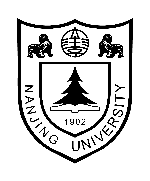
\includegraphics[width=1.96cm]{logo} \\
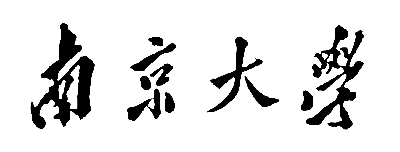
\includegraphics[height=2cm]{name} \\
\vskip 1cm
\zs
\zihao{0} 硕~~士~~毕~~业~~论~~文\\
\vskip 2in\zihao{3}
\begin{minipage}{0.9\textwidth}
院\qquad 系\NJUTunderline{\department}\\[3mm]
专\qquad 业\NJUTunderline{\major}\\[3mm]
题\qquad 目\NJUTunderline{\thesistitle}\\[3mm]
年\qquad 级\myuline{4.5cm}{\grade}{\hfill}学\qquad 号\myuline{4cm}{\NJUID}\\[3mm]
学生姓名\NJUTunderline{\myname}\\[3mm]
指导老师\myuline{4.5cm}{\advisor}{\hfill}职\qquad 称\myuline{4cm}{\advisorjob}\\[3mm]
论文提交日期\NJUTunderline{\today}
\end{minipage}
\end{center}
\clearpage
\thispagestyle{empty}
\vspace*{\stretch{1}}
{\kai\zihao{-3}
\noindent
\begin{tabular}{lll}
\begin{CJKfilltwosides}{3.5cm}学号\end{CJKfilltwosides} & : & \makebox[6cm][l]{\NJUID}\\
\begin{CJKfilltwosides}{3.5cm}论文答辩日期\end{CJKfilltwosides} & : & \uline{\qquad}年\uline{\quad}月\uline{\quad}日\\
\begin{CJKfilltwosides}{3.5cm}指导教师\end{CJKfilltwosides} & : & \uline{\qquad\qquad\quad}(签字)\\
\end{tabular}
}
}

\newcommand\makeenglishtitle{%
\clearpage
\thispagestyle{empty}
\begin{center}
\vspace*{20pt}
\bf\zihao{2} \ethesistitle
\vskip \stretch{1}
\normalfont\zihao{4} by
\vskip 3pt
\bf\zihao{4} \emyname
\vskip \stretch{1}
\normalfont\zihao{4} Directed by
\vskip 3pt
\bf\zihao{4} \eadvisor
\vskip \stretch{2}
\normalfont\large \edepartment \\Nanjing University
\vskip 30pt
\CTEXoptions[today=old]
\normalfont\large \today
\vskip 20pt
\it\large Submitted in full fulfilment of the requirements\\for the degree of Bachelor of Computer Science and Technology.
\end{center}
}

\setlength{\headheight}{15pt}

\begin{document}
\frontmatter
\normalfont
% !Mode:: "Tex:UTF-8"
\begin{abstract}

\end{abstract}

\keywords{多标签;层次;法律适用;识别}

\begin{englishabstract}

\end{englishabstract}

\englishkeywords{Multi-label;Hierarchy;Application of Law; Recognition}
\clearpage

\pdfbookmark[0]{目录}{tableofcontents}
\tableofcontents
%\listoffigures
%\listoftables  这条命令是表格目录,需要的话可以启用;上面那条是图片目录,不需要可以注释掉或者直接删除

\mainmatter
\zihao{-4}
\song
% !Mode:: "Tex:UTF-8"\chapter{Introduction}
\chapter{绪论}

    \section{研究背景及意义}
    随着我国法治建设的逐步推进,人民的法律意识日渐提高,人们在遇到争议事件时会更多地选择诉诸法律,以公平公正地解决问题。根据最高人民法院的数据,2015年全国各级法院审结一审民事案件达622.8万件。然而,由于法律的专业性和复杂性,普通民众自身在借助法律维护自身权益的时候往往无所适从,只能求助律师等专业人士;另一方面,法律条文浩如烟海,即便是专业律师也只能专注于某一领域,在面对不熟悉的法律条文或者案例时,也需要一些决策辅助。

    信息技术,尤其是信息检索和数据挖掘技术的发展,为法律辅助系统的实现提供了可能。“北大法宝”、“找法网”等一批在线法律信息平台,提供了法规案例检索、律师推荐等功能,在一定程度上为人们诉诸法律解决争端提供了便利。然而,上述平台提供的服务并未直接解决人们的问题。法规案例的检索往往需要用户有明确的搜索目标,甚至需要一定的法律领域知识,而且即便搜索引擎能够给出相应的搜索结果,这些结果通常也无法直接解决用户的问题,需要用户自己的分析和理解。律师推荐能够方便用户找到合适的律师,实际上是连接用户和律师的桥梁,不仅无法提供问题的直接解决方案,还容易受商业化的影响,出现一些律师滥竽充数的情况。

    随着我国司法公开改革的推进以及最高人民法院关于人民法院在互联网公布裁判文书的规定的实施,蕴藏了海量信息的裁判文书可以方便地被获取和分析。2014年以来,全国各级法院共在“中国裁判文书网”上传裁判文书六百余万份,最高人民法院和部分省市区法院实现了能够上网的生效裁判文书全部上网的目标。裁判文书记载了人民法院审理案件的过程和结果,是诉讼活动结果的载体,也是人民法院确定和分配当事人实体权利义务的惟一凭证。一份结构完整、要素齐全、逻辑严谨的裁判文书,既是当事人享有权利和负担义务的凭证,也是上级人民法院监督下级人民法院民事审判活动的重要依据。因此,裁判文书中包含的当事人诉求、犯罪行为、行政执法、司法裁判行为和过程、法律的适用等信息,作为重要的历史数据,通过数据挖掘手段进行分析,可以为司法人员、律师和普通民众提供必要的决策支持。\cite{向李兴2015基于自然语义处理的裁判文书推荐系统设计与实现}实现了一个裁判文书推荐系统,为法官提供与当前裁判文书相似的文书,作为裁判的参考。基于自然语言处理技术提取文书的语义信息,在裁判文书的相似度计算上取得了不错的效果。裁判文书推荐可以提供决策辅助,但是逐条查阅相似案例需要耗费大量精力,同时由于案例相似度不同,需要用户自行确定各个案例的权重进行综合评判,极大地降低了查询结果的直观性和明确性。

    从本质上讲,裁判是法院依照法律,对案件做出决定的过程。“以事实为根据,以法律为准绳”是我国社会主义法律适用遵循的基本原则,司法机关处理一切案件,都是根据客观事实,以国家法律为标准和尺度。因此,根据案件的描述确定适用的法律,是法院判决过程的核心部分,也是律师和普通民众在法律活动中需要解决的首要问题。运用信息技术,根据案件事实描述实现适用法律的自动识别,将在很大程度上为人们的法律活动提供更加直接和明确的帮助。现已公开的裁判文书中包含的案件事实描述以及法律适用信息,为我们提供了大量的带标签数据集,采取合适的数据挖掘手段,可以从中学习得到有效的预测模型,实现对未判案件适用法律的自动识别。


    \section{研究内容及目标}
    本文希望通过运用数据挖掘方法,从海量的裁判文书中,学习出由案件事实描述到适用法律的预测模型,从而为用户提供直接的法律决策辅助。

    一份结构完整的裁判文书包括首部、事实、理由、裁判结果和尾部,其中首部包括裁判文书的类型、编号、裁判法院,案件当事人、委托代理人等信息,事实部分包含了对案件事实的描述,理由部分阐述了法院对于案件的分析以及做出相应裁判结果的理由,裁判结果部分给出了法院对于此次诉讼的判决或裁定结果,尾部则包含了审判人员、时间等信息。

    运用数据挖掘手段进行案件适用法律的自动识别,首先需要提取能够充分描述案件事实的特征,由于裁判文书及其中的事实描述部分主要是以文本形式存在,因此需要运用到文本挖掘技术\cite{aggarwal2012mining},包括中文分词,文本表示,特征选择和特征权重计算等。

    本文通过监督式学习方法来构建预测模型,样本的标签即为案件适用的法律条文,包含在裁判文书中的裁判理由部分。由于裁判文书格式的不规范性,裁判文书引用法律条文的格式没有统一格式,因此需要对提取的案件适用的法律条文作进一步处理,形成数据集的标签。与传统的分类问题不同的是,一份裁判文书中往往包含多个法律条文的引用,因此法律适用的自动识别问题是一个多标签分类问题\cite{tsoumakas2006multi}。在多标签学习中,每个样本可以对应多个标签,使得学习问题更加复杂。更进一步地,法律条文的组织呈现为树状结构,如图\ref{Figure1}所示。一个案件不仅可能适用多项法律条文,这些法律条文的具体程度也可能不同,即案件适用的法律条文可能位于树结构的叶节点,也可能位于树结构的内部节点。如果忽略法律条文的树形结构特征,无疑会损失分类标签的重要信息,造成预测模型性能的下降。因此,如何利用标签的结构信息,是本文的重要研究内容。本质上,法律适用自动识别问题是一个层次多标签学习问题\cite{barutcuoglu2006hierarchical},其中样本的特征需要通过文本挖掘手段从文本中提取,而标签的结构呈树形。
    
    \begin{figure}[ht]
        \centering
        % Requires \usepackage{graphicx}
        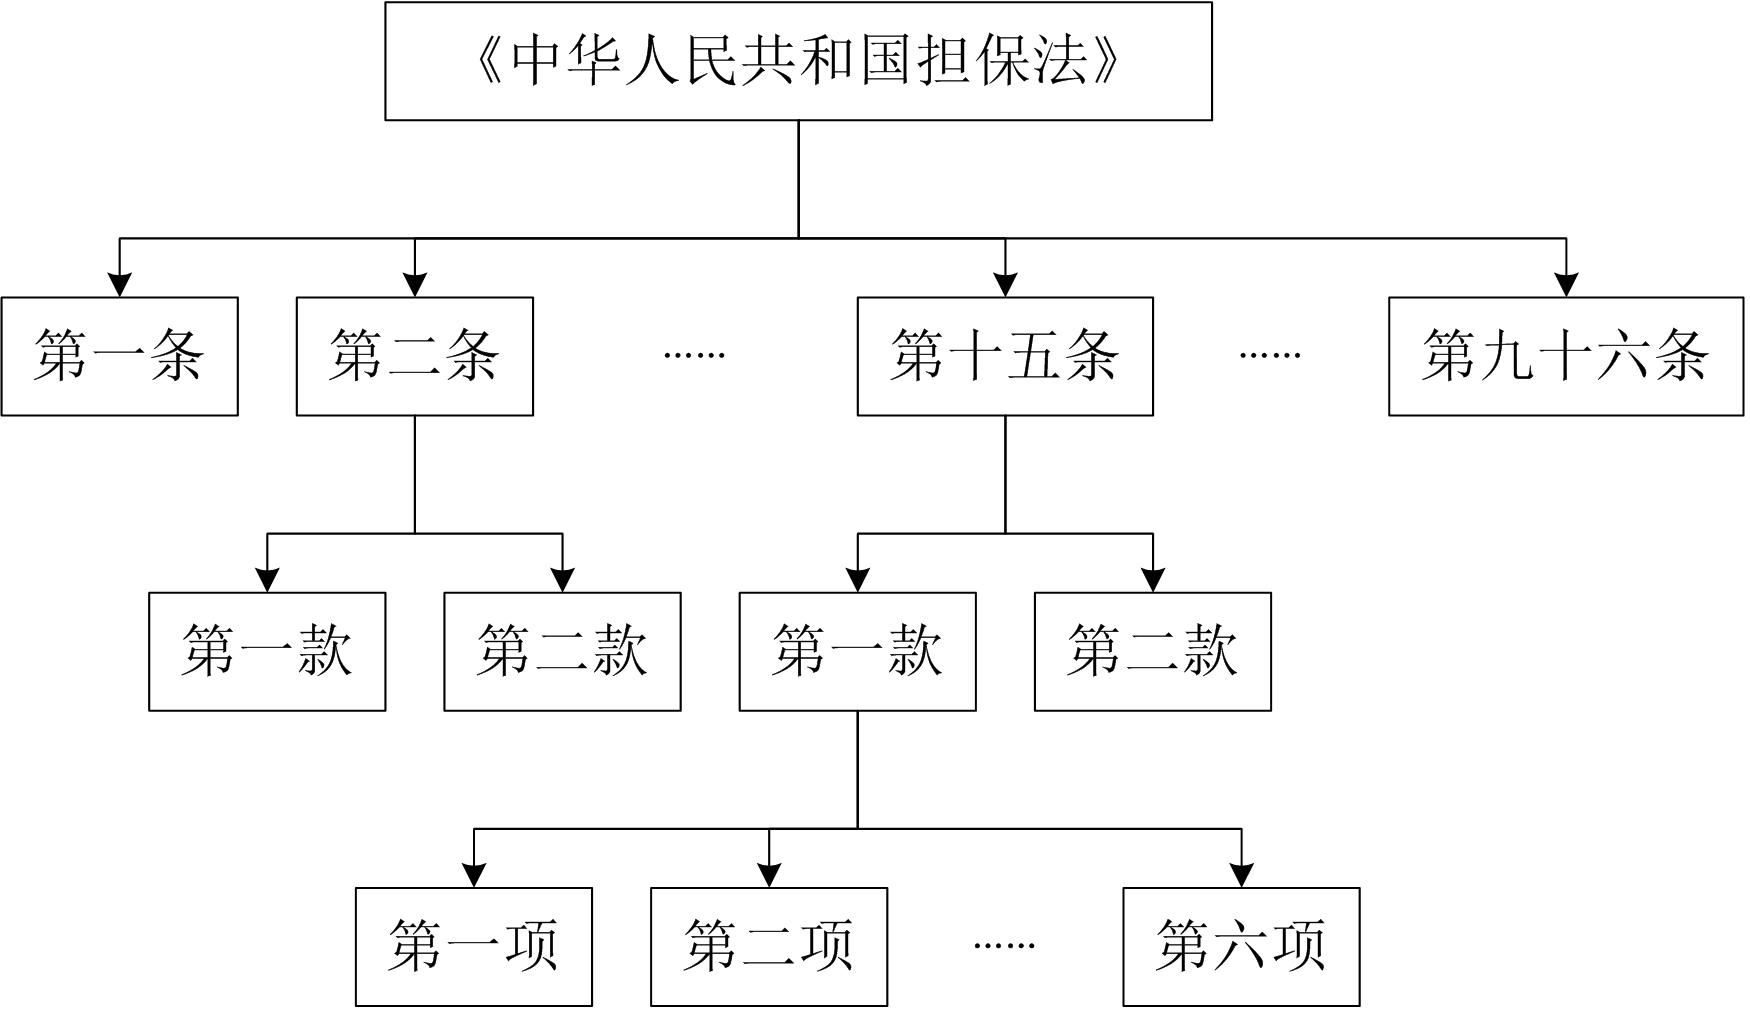
\includegraphics[width=10cm]{Figure1}\\
        \caption{法律条文树形结构示例}\label{Figure1}
    \end{figure}
    
    综上,本文研究的目标是解决案件适用法律的自动识别问题,研究的方法是首先利用文本挖掘技术对海量裁判文书进行处理分析,得到案件事实的结构化表示,即样本特征,数据集中的每个样本可以对应于标签空间中的多个标签,标签空间以树状结构组织。在此数据集上通过层次多标签学习构建预测模型,实现对未判案件适用法律的识别。


    \section{论文组织}
    本文组织如下:

    第一章介绍本文研究的背景和意义,阐述法律适用自动识别在当前民众法律活动中的重要辅助作用,并提出研究内容和目标,指出面临的问题及解决方向。

    第二章为相关技术部分,主要对本文研究涉及的文本挖掘技术、层次多标签学习技术和非平衡分类问题进行介绍,主要对已有的层次多标签学习的工作进行综述。

    第三章详述本文提出的LocalBalance层次多标签学习算法。

    第四章为实验部分,包括本文数据集的构建,即利用文本挖掘技术对海量裁判文书进行处理,构建结构化数据集的过程,以及运用本文算法训练得到的模型的性能分析。

    第五章对本文工作进行总结,并提出改进的方向。

%% !Mode:: "Tex:UTF-8"\chapter{Related work}
\chapter{相关技术}
    本文主要研究基于DAPro 平台的分布式算法实现,与本文相关的工作主要包括其他相关网络模拟平台和离散事件模拟两个方面。下面我们对这两个方面的工作进行简要介绍,并分析其与本文工作的联系和区别。

    \section{网络模拟平台}
    NS2(Network Simulator, version 2)是一款开放源代码的网络仿真软件。它最初为了研究大规模网络以及当前和未来的网络协议交互行为而开发。它为有线和无线网络上的TCP、路由和多播等协议的仿真提供了强有力的支持。NS2 是一个开源项目,所有源代码都开放,任何人可以获得、使用和修改其源代码。正因为如此,世界各地的研究人员每天都在扩展和更新它的功能,为其添加新的协议支持和功能模块。它也是目前网络研究领域应用最广泛的网络仿真软件之一。

    NS2 是一种面向对象的网络仿真器,本质上是一个离散事件模拟器,由UC Berkeley 开发而成。它本身有一个虚拟时钟,所有的仿真都由离散事件驱动的。目前NS2 可以用于仿真各种不同的通信网络,已经实现的一些仿真模块有:网络传输协议,比如TCP 和UDP;业务源流量产生器,比如FTP,Telnet,Web CBR 和VBR;路由队列管理机制,比如Droptail,RED和CBQ;路由算法,比如Dijkstra 等。NS2也为进行局域网的仿真而实现了多播以及一些MAC 子层协议\cite{ns2introduction}。

    然而,NS2 的内容过于庞杂,并且主要面向网络模拟,并非针对分布式算法的设计实现和测试。同时由于需要了解大量相关知识和工具,NS2 对于用户而言难于掌握。本文介绍和使用的DAPro 平台更为精简,专门针对于分布式算法的模拟。用户可以在短时间内掌握平台的基本结构,利用平台进行分布式算法的设计、实现和测试,也可以在遵守DAPro 设计规范的基础上自行扩充其功能,满足自身设计需求。

    \section{离散事件模拟}
    在模拟仿真领域,离散事件模拟将系统的操作建模为基于时间的离散事件序列。每个事件在某个特定瞬间适时发生,并引发系统状态的一个改变\cite{robinson2004simulation}。在连续的事件之间,假定系统不发生任何改变。因此,仿真能够从一个事件适时地转到下一个事件。

    DES 系统通常包含以下几个组件(Component):
    \begin{enumerate}
    \item Clock,时间。系统时间是离散的,可以使用初值为0,不断递增推进的整数序列来模拟。时间为DES 其他组件所共享。比如,事件(Event)会带有时间标签,表明其何时应该被调度。系统引擎(Engine) 会根据被模拟的场景逻辑计算或者判断何时应该产生新的事件,何时应该调度某事件等。
    \item Event,事件。事件是一个DES 系统的核心概念。设计DES 系统,需要明确定义在该系统中哪些行为被视为事件。事件可以具有逻辑上的分类,比如有消息事件(发送消息事件、接收消息事件),延时事件(随机延时、定时延时等)和异常事件(节点失效事件)等。
    \item Eventlist,事件列表。事件带有时间标签,所有的事件通常按照时间先后顺序排列在事件列表中,以等待系统引擎(Engine) 调度执行。事件列表通常使用优先级队列来实现。
    \item Engine,引擎。引擎是DES 系统的控制部件。它负责系统的启动、运行和终止。启动时通常会产生初始事件;系统运行期间不断产生新的事件并调度执行;引擎会判断终止条件是否成立。
    \end{enumerate}

    离散事件模拟的应用十分广泛,DAPro 平台正是基于离散事件模拟设计实现的,系统由一系列离散事件驱动。事实上,离散事件模拟的研究为众多模拟软件提供了理论基础,包括上文中的NS2 网络模拟平台。

%% !Mode:: "Tex:UTF-8"
\chapter{分布式计算理论基础}
    本章主要介绍有关分布式计算模型的一些基础理论知识。我们将首先介绍消息传递系统形式模型,包括异步和同步两种消息传递系统,之后我们会讨论在系统可容错情况下的故障模型。

    \section{消息传递系统}
    在消息传递系统中,处理器之间的通信通过在通信信道上发送消息实现。每个信道在两个特定的处理器之间建立一条双向连接。通信信道的连接情况描述了系统的拓扑结构。系统拓扑由一个无向图表示,其中每个节点代表一个处理器,当且仅当两个节点所对应的处理器之间存在信道时,这两个节点之间的边才存在。我们目前只考虑系统拓扑为连通图的情况。通常,我们将信道的集合称为网络。具有特定拓扑的消息传递系统中,一个算法由系统中的每个处理器的本地程序组成。一个处理器的本地程序使得处理器能够执行本地计算,向给定拓扑中的邻居发送消息,以及接收来自邻居的消息。
    \begin{figure}[ht]
        \centering
        % Requires \usepackage{graphicx}
        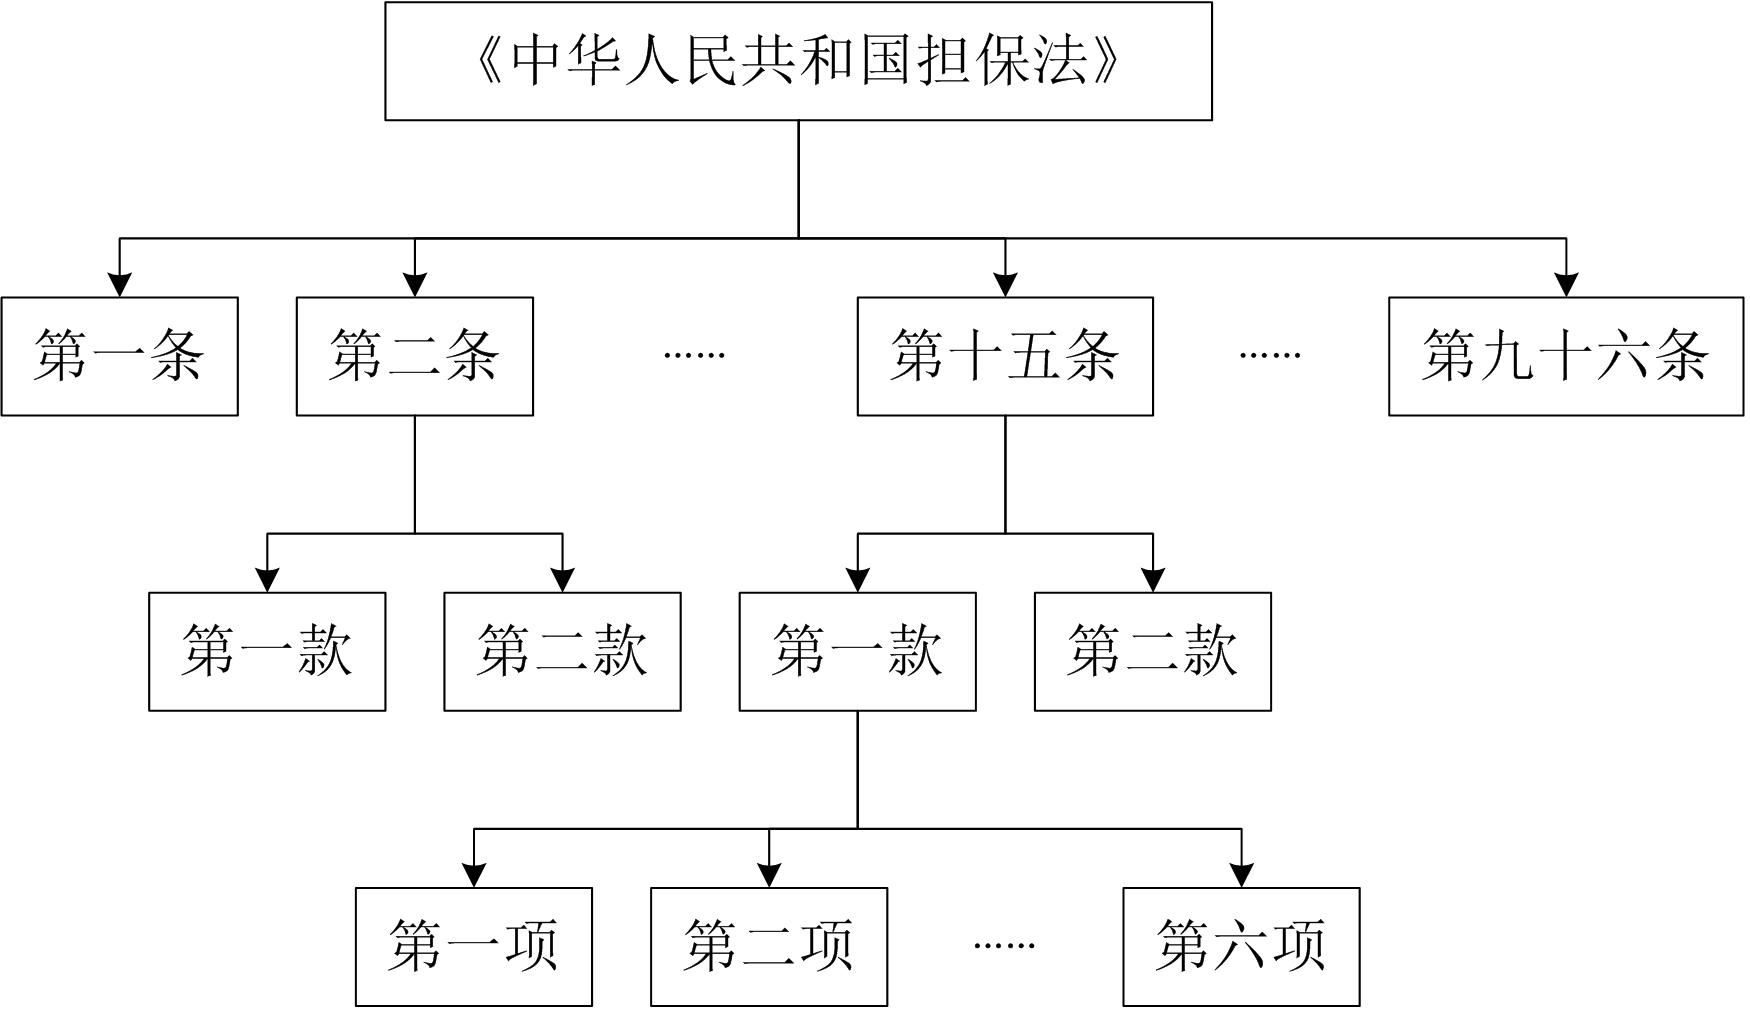
\includegraphics[width=10cm]{Figure1}\\
        \caption{一个简单的拓扑图}\label{Figure1}
    \end{figure}

    更正式地讲,一个系统或者算法由$n$ 个处理器$p_0,...,p_{n-1}$ 组成,其中$i$ 是处理器 $p_i$ 的索引。每个处理器$p_i$ 被建模为一个(可能是无限的)状态机,其状态集合为$Q_i$\cite{lynch1981describing}。一个处理器在拓扑图中被标识为一个特定的节点。拓扑图中与处理器$p_i$ 邻接的边被随机标注为整数$1$ 到$r$,其中$r$ 是$p_i$ 的度(见图\ref{Figure1})。处理器$p_i$ 的每个状态包含$2r$ 个特殊组件,$outbuf_i[l]$ 和$inbuf_i[l]$,其中每个$l$ 均满足$1 \leq l \leq r$。 这些特殊的组件是消息的集合:$outbuf_i[l]$ 保存了$p_i$ 通过第$l$ 条邻接信道发送给邻居但是尚未被交付的消息,$inbuf_i[l]$ 保存了通过第$l$ 条邻接信道交付给$p_i$ 但是$p_i$ 尚未通过内部计算步骤进行处理的消息。状态集合$Q_i$ 含有一个特殊的子集$\pozhehao$初始状态。在初始状态中,每个$inbuf_i[l]$ 必须为空,而$outbuf_i[l]$ 组件并不需要。

    处理器的状态,除去$outbuf_i[l]$ 组件,组成了$p_i$ 的可容许状态(admissible state)。当向$p_i$ 的可容许状态输入一个值时,处理器$p_i$ 的转换函数开始执行。执行的结果是为$p_i$ 的可容许状态输出一个值,该状态中每个$inbuf_i[l]$ 为空。执行的结果也可能是为每一个$1$ 到$r$ 之间的$l$ 输出最多一条消息:这就是将要发送给在$p_i$ 的第$l$ 条邻接信道另一端的邻居的消息。因此,$p_i$ 之前发送并等待交付的消息不会影响$p_i$ 当前的步骤;每个步骤处理所有等待交付给$p_i$ 的消息并且引发状态的改变,同时会向每个邻居最多发送一条消息。

    一个配置(configuration)是一个矢量$C=(q_0,...,q_{n-1})$ ,其中$q_i$ 是$p_i$ 的一个状态。一个配置中$outbuf$ 的状态表示了通信信道上正在传送的消息。一个初始配置是一个矢量($q_0,...q_{n-1}$),其中每个$q_i$ 是$p_i$ 的一个初始状态,也就是说,每个处理器都处在初始状态。

    系统中能够发生的动作被建模为事件。对于消息传递系统,我们考虑两种事件。一种是计算事件,表示为$comp(i)$, 代表处理器$p_i$ 的一次计算步骤,该步骤中$p_i$ 的转换函数会应用到它当前的可容许状态。另一种是交付事件,表示为$del(i,j,m)$,代表消息$m$ 从处理器$p_i$ 发送到$p_j$。

    系统随时间的行为被建模为执行(execution),即为一个配置和事件相交替的序列\cite{owicki1976axiomatic}。这个序列要满足各种各样的条件,这些条件由被建模系统的特定类型决定。我们将这些条件分为安全性和活跃性条件两类。安全性条件要求序列的每个有限前缀都要满足;比如,“处理器$p_i$ 的每一个步骤之后都跟随着处理器$p_0$ 的一个步骤。”非正式地讲,安全性条件声明了系统中还没有坏事发生;比如刚刚给的例子可以重新描述为要求$p_1$ 的一个步骤之后绝不会跟随着除了$p_0$ 之外的其他处理器的一个步骤。活跃性条件是必须保持一个特定次数,可能是无限次的条件。例如,条件“$p_1$ 进行无限次步骤”需要条件“$p_1$ 刚刚进行一次步骤”必须重复发生无限次。非正式地讲,活跃性条件表示最终有些好事发生。满足一个特定系统类型要求的所有安全性条件的任意序列可以称为执行。如果一个执行也满足所有要求的活跃性条件,那么它是可容许的\cite{fischer1985impossibility}。

    下面我们来定义同步和异步这两种消息传递系统中的执行和可容许执行需要满足的条件。

    \subsection{异步消息传递系统}
    对于一个系统,如果消息传递花费的时间以及处理器的连续步骤间的时间间隔没有固定的上限,那么这个系统就称为是异步的。异步系统的一个例子就是因特网,消息(比如E-mail)可能会过几天才能到达,尽管这经常只需要数秒。通常消息延迟和处理器步骤时间间隔会有上限,但是有时候这些上限会很大,只会在极少的情况下达到,而且会随着时间变化。我们通常需要设计独立于任何时间参数而不是依赖于这些限制的算法,也就是异步算法。

    异步消息传递系统中的一个执行片段$\alpha$ 是一个如下形式的(有穷或者无穷的)序列:
    \begin{center}
    $C_0,\phi_1,C_1,\phi_2,C_2,\phi_3,...$
    \end{center}

    其中每个$C_k$ 是一个配置,每个$\phi_k$ 是一个事件。如果$\alpha$ 是有限的,那么它必须以一个配置结束。进一步地,以下条件必须满足:
    \begin{itemize}
      \item 如果$\phi_k=del(i,j,m)$,那么$m$ 必须是$C_{k-1}$ 中$outbuf_i[l]$ 的一个元素,其中$l$ 是$p_i$ 赋予信道$\{p_i,p_j\}$ 的标签。从配置$C_{k-1}$ 到$C_k$ 的唯一变化是$m$ 从$C_{k-1}$ 中的$outbuf_i[l]$ 中移除,同时$m$ 被加入到$C_k$ 中的$inbuf_j[h]$,其中$h$ 是$p_j$赋予信道$\{p_i,p_j\}$ 的标签。总之,一条消息被交付当且仅当它处于发送状态,并且发生的唯一变化是把消息从发送方的输出缓冲移动到接收方的输入缓冲。
      \item 如果$\phi_k=comp(i)$,那么从$C_{k-1}$ 到$C_k$ 的唯一变化是$p_i$ 根据其作用于$C_{k-1}$ 中$p_i$ 的可容许状态上的转换函数改变状态,同时由$p_i$的转换函数确定的消息集合会被加入到$C_k$ 中的$outbuf_i$ 参数中。这些消息被称作在这个事件中被发送。总之,$p_i$ 基于其当前状态由转换函数(本地程序)改变状态并发送消息,当前状态包含了待交付的消息(但不包括待发送消息)。处理器的转换函数会保证$inbuf$ 变量会被清空。
    \end{itemize}

    一个执行(execution)是一个执行片段$C_0,\phi_1,C_1,\phi_2,C_2,\phi_3,...$,其中$C_0$ 是初始配置。

    对于每个执行(或者执行片段)我们关联一个计划(或者计划片段),所谓计划(schedule)即为执行中事件的序列,$\phi_1,\phi_2,\phi_3,...$。不是每个事件序列都能与每个初始配置相匹配:比如,$del(1,2,m)$ 不是$outbufs$ 为空的初始配置的一个计划,因为没有$p_1$ 的之前的步骤能导致$m$ 被发送。注意如果本地程序是确定性的,那么执行(或者执行片段)就只由初始(或开始)配置$C_0$ 和计划(或者计划片段)$\sigma$ 决定,表示为$exec(C_0,\sigma)$。

    在异步模型中,一个执行是可容许的当且仅当每个处理器都执行无穷次计算事件并且发送的每条消息都最终被交付。要求无穷次计算事件模拟了处理器不会发生故障的事实。它不代表处理器的本地程序必须包含一个无限循环;一个算法结束的非正式概念可以调整为一旦处理器完成了它的任务,使其转换函数在一个特定的点之后不再改变处理器的状态。换句话说,处理器在那个时间点之后执行“假步骤”。如果一个计划是一个可容许执行的计划,那么它是可容许的。

    \subsection{同步消息传递系统}
    在同步系统中,处理器按照锁步(lockstep)执行:一个执行被分割成若干时间片,在每个时间片,每个处理器可以向每个邻居发送一条消息,所有消息将被交付,之后每个处理器会根据刚刚收到的消息进行计算。这种模型,在实际的分布式系统中尽管通常无法达到,但是对于算法设计非常方便,因为算法不需要考虑很多不确定性。当一个算法针对这一理想的时间模型设计之后,可以自动模拟到其他更为现实的时间模型中工作,正如我们接下来将要看到的一样。

    正式地讲,同步情况下执行的定义比起异步情况下的定义有了进一步的限制,其定义如下。间隔的配置和事件可以被分割成不相交的周期(round)。 一个周期包含了$outbuf$ 变量中所有消息的一次交付事件,直到所有的$outbuf$ 变量为空,紧接着所有处理器进行一次计算。因此,一个周期包含了如下过程:首先交付所有待发送的消息,然后让所有的处理器进行一次内部计算步骤来处理所有交付了的消息。

    同步模型中,如果一个执行是无限的,那么它是可容许的。由于周期的结构,这意味着每个处理器进行无限次计算步骤,并且每条发送的消息最终都会被交付。在异步的情形下,假定可容许执行是无限的是为了追求技术上的便利;同步情形下算法的终止可以像异步情形中一样处理。

    注意在没有故障的同步系统中,一旦算法确定,执行能够不同的唯一影响因素是初始配置。在异步系统中,同一算法会有很多不同的执行,即便是初始配置相同且没有故障,这是因为处理器步骤之间可以交叉并且消息延迟是不确定的。

    \section{故障模型}
    当分布式系统不可靠时,会产生很多新的问题。对于同步消息传递系统中的良性故障,一个错误的处理器会崩溃,也就是停止运行,但是不会执行错误的操作(例如交付尚未被发送的消息)。我们研究一个基本的协同问题$\pozhehao$协商问题,它需要所有的处理器根据它们的(可能冲突的)输入达成一个共同的输出。还是在同步消息传递系统中,错误的处理器可能产生有更为严重的错误行为。我们假定故障是拜占庭的(Byzantine),也就是一个发生故障的处理器的行为是任意的。在这种情况下如果要解决协商问题,错误的处理器数量不能多于总数的三分之一。而在异步系统中,一个确定性算法无法解决协商问题,即便只有一个处理器以简单崩溃的形式发生故障。不管通信是以消息传递还是共享读写变量实现,这一结论都成立。

    我们要讨论的是容错分布式计算中的一个简单例子:一个同步系统,其中处理器会以简单地停止运行方式发生故障。我们假定对于我们讨论的所有消息传递系统,其通信拓扑图是完全的,即处理器都处于一个环的节点上。更进一步地,我们假定通信信道完全可依赖,所有发送的消息都将被交付。

    为了应对处理器崩溃的情况,我们需要修改同步消息传递系统中一些形式定义。在定义中一个至关重要的参数是$f$,也即能够失效的处理器的最大数量。我们称这样的系统是$f-resilient$ 的。

    在系统可靠的情况下,同步系统的一个执行由一系列的周期组成。在每一周期,$outbuf$ 变量中的所有消息都会被交付,然后所有处理器都将进行一次运算。而对于一个$f-resilient$ 系统,一个执行的定义修改如下。存在一个包含$f$ 个处理器的子集$F$,即错误处理器集合。错误处理器集合在不同执行中可能不同,因此我们无法提前知道哪个处理器是错误的。在每个周期中,每个不在$F$ 中的处理器都正好有一次计算事件,而在$F$ 中的处理器最多有一次计算事件。更进一步地,如果$F$ 中的某个处理器在某个周期没有计算事件,那么在任何后继周期中也不会有计算事件。最后,在一个错误处理器执行计算事件的最后一个周期,其输出消息集合中的一个随机子集会被发送\cite{attiya2004distributed}。

%% !Mode:: "Tex:UTF-8"
\chapter{DAPro 平台的设计与实现}
    DAPro,全称Distributed Algorithm Fast Prototyping Platform,旨在为分布式算法的设计、实现以及测试提供一个快速原型平台。DAPro 是基于Discrete Event Simulation(离散事件模拟,以下简称为DES) 理念而设计的。在DES 中,系统的运作是由一系列在离散时间发生的事件所驱动的。DAPro 的设计是面向分布式算法的,我们目前采用分布式计算中的消息传递模型(Message Passing Model)。

    \section{DAPro 总体概述}
    总体概述部分将对DAPro 的主要模块和运行流程进行介绍。DAPro 包括了Event、Engine、System、Communication 和FailureGenerator 模块,DAPro 的运行流程揭示了模块间的调用关系。

    DAPro 主要由如下几个模块构成,各模块的功能和大体实现描述如下:
    \begin{description}
        \item[Event] Event 的定义包含两个要素,一为Event 的触发时间(triggeringClock),二为Event 的处理函数(IEventHandler 实例)。在实例化一个Event 对象时,需要确定以上两个参数。事件的触发时间可以相同,表示事件同时执行。
            
            凡是需要处理Event 的实体(SimulationObject 实例)均需要实现IEventHandler 接口,并实现其中的dispatch(Event e) 抽象方法用以对Event 做任何必要的处理。
            
            IEventCollection 是EventList(事件列表)的抽象实现,PQEventCollection 是EventList 的优先级队列版本的具体实现。
        
        \item[Engine] Engine 采用Singleton 模式,实现了DES 的核心控制功能,其主要逻辑由方法run 实现:
            \begin{itemize}
                \item 从EventList 中取出下一个事件e,这也是即将要调度执行的事件。
                \item 将模拟时钟Clock 推进到事件e 的triggeringClock,表示即将执行该事件。
                \item 调用事件的action 方法将事件交由其IEventHandler 处理。
            \end{itemize}
            
            Engine 会重复以上步骤,直到模拟时钟超过了最大允许时间或事件列表为空。
            
            在事件e 的执行过程中,可能产生新的事件。新产生的事件需要加入到事件列表中,以便Engine 调度执行。事件的加入有两种方式,scheduleEvent() 和scheduleEventAtOnce(),前者会将事件延迟一个固定或者随机的时间,后者会将事件直接加入事件列表,不改变事件的处理时间。
        
        \item[System] System 包含了系统的拓扑结构和组成要素,系统拓扑由进程\footnote{根据Nancy Lynch《分布式算法》:“It is often useful to think of them (computing elements) instead as logical software ‘processes’, running on (but not identical to) the actual hardware processors.”}节点和节点间的连接关系组成。
            \begin{figure}[ht]
                \centering
                % Requires \usepackage{graphicx}
                \includegraphics[width=10cm]{SystemTopology}\\
                \caption{系统拓扑图}\label{SystemTopology}
            \end{figure}
            
            DAPro 对系统拓扑的描述见图\ref{SystemTopology}。其中:
            \begin{itemize}
                \item Process 对象是事件的执行实体。系统拓扑中的每个节点都表示一个进程,每个进程都有一个独一无二的标识符,系统中使用自然数来表示。进程用于存储信息以及对事件进行处理。
                \item Link 对象表示信道,负责消息的传递。Link 对象由Connector 对象以链表的形式组装而成。在此结构的基础上,Connector 负责最底层信息处理,不同类型的Connector 可以模拟实现网络通信的不同特性。
                \item Session 对象维护了两个进程及其连接两者的信道,即进程fromProcess、toProcess 和信道link。当两个进程需要通信时,可以通过Session 找到相应的信道,进行信息的传输。
                \item System 负责建立、维护和查询系统拓扑。系统拓扑包含Process 和Session 两部分,System 使用id2Process 和pair2Session 两个HashMap 数据结构来表示系统拓扑结构。
            \end{itemize}
        
        \item[Communication] 系统中进程间通信由Communication 完成。Communication 实现了消息传递系统中消息发送功能的封装,包括创建消息事件,并将该事件加入到事件列表交由Engine 调度。Communication 需要找到消息发送方与接收方的信道,实现消息的传递,从而最终将消息事件交付到接收方执行。
        
        \item[FailureGenerator] FailureGenerator 是DAPro 的故障产生模块,用于模拟产生不可靠系统中可能出现的各类故障,包括崩溃故障、拜占庭故障等。故障的模拟也是通过创建故障事件,交由相应的进程处理。系统中故障的数量可能会有限制,因此需要相应地对故障的产生进行控制。
    \end{description}

    DAPro 的运行需要各个模块相互协调,共同作用。系统的核心是事件(Event),事件由系统引擎(Engine)调度,交由相应的事件处理实体执行;进程之间的通信由通信(Communication)模块完成,Communication 需要查询系统拓扑(System),将消息通过信道传递到目标进程,从而完成进程间的消息传递。

    \section{DAPro 各模块详细设计}
    本节我们讨论DAPro 系统的模块设计。根据总体概述中的模块划分,我们会依次对系统中每个模块的功能和实现进行详细分析。

    \subsection{Event 模块}
    Event 模块是DAPro 系统核心模块之一,事件是整个系统的核心概念。Event 模块中包含了Event 类及其子类,构成了系统能够模拟的事件的集合,其类图如图\ref{Event}所示。

    \begin{figure}[ht]
        \centering
        % Requires \usepackage{graphicx}
        \includegraphics[width=14cm]{Event}\\
        \caption{Event 模块类图}\label{Event}
    \end{figure}

    下面我们分别对模块中的类和接口的功能和实现进行说明:
    \begin{description}
      \item[Event] 所有Event 类均含有参数触发时间triggeringClock 和处理实体handler。事件被执行的顺序由触发时间决定,通过在事件触发时间上加上一定的延迟可以对事件执行顺序进行调度;而事件的处理实体决定了事件交由何种实体处理。一个事件被Engine 调度后,会首先调用其action 方法,将该事件交付给其处理实体进行处理。注意action 方法被定义为final,因此Event 的子类不能覆盖该方法,action 方法的全部功能即为调用handler 的dispatch 方法对事件进行处理。
      \item[IEventHandler] IEventHandler 接口是所有能够对事件进行处理的实体的抽象。系统中的Process、Session、Link 等类均需要实现该接口,并实现其中的dispatch 方法对事件进行相应处理。
      \item[ProcessStartEvent] ProcessStartEvent 是一种特殊的事件,用于某些类型进程的启动。除了继承Event 类的特性和操作外,它不具备其他内容。ProcessStartEvent 事件一般与ProcessStartAction 相对应。
      \item[MessageEvent] 在消息传递系统中,最为常见的事件是消息事件。除了事件的触发时间和处理实体,MessageEvent 类中还包含了消息内容、消息的发送方和消息的接收方。进程对象通过接收处理消息事件来接收消息,并借助Communication 模块创建消息事件发送消息,从而可以实现进程之间的信息交互。
          
          DAPro 系统中各种类型的消息由Message 类及其子类表示。Message 类是一个基类,我们可以通过继承Message 类定义更为复杂的消息类型。SpanningTreeMessage 类和ConsensusMessage 类都是针对具体问题定义的消息类型,我们会在后面的实现部分具体分析。
      \item[RoundEvent] 在同步系统中,进程的运行是以周期为单位的。DAPro 系统中,进程按周期执行是通过接收处理相应的RoundEvent 实现的。进程接收到一个RoundEvent,即表示一个新的周期开始。在每个周期中,消息发送和本地计算环节可能需要分隔开,因此我们定义了RoundEvent 的两个子类:MessagePassingRoundEvent 类和LocalComputationRoundEvent 类,前者代表一个周期中的消息发送环节,后者代表一个周期中的本地计算环节,两者共同构成了一个完整的周期。除了继承Event 的特性,RoundEvent 还包含有roundNo 参数表示周期编号,有些进程对象需要根据周期编号来决定其行为。
    \end{description}

    \subsection{Engine 模块}
    Engine 模块同样是DAPro 系统核心模块之一,采用单例模式实现。作为系统的引擎,Engine 模块控制事件的调度执行,其模块类图如图\ref{Engine}。
    \begin{figure}[ht]
        \centering
        % Requires \usepackage{graphicx}
        \includegraphics[width=14cm]{Engine}\\
        \caption{Engine 模块类图}\label{Engine}
    \end{figure}

    Engine 维护了一个全局的系统时间和一个事件列表,系统时间是事件调度运行的时间依据,而事件列表保存了Engine 能够调度的事件集合。Engine 主要完成的工作是事件的调度执行,事件的调度由scheduleEvent 和scheduleEventAtOnce 两个方法实现,而事件的执行由run 方法实现。事件调度的两种方法主要逻辑相同,即将要调度的事件插入到事件列表中,区别在于scheduleEvent 能够为事件的触发时间加上一个延迟。系统通过调用Engine 的run 方法开始运行,从事件列表中取出事件,更新系统时间并执行该事件,系统会重复这一行为直到事件列表为空或者系统时间到达上限。

    事件列表的实现可以有多种,但至少要包括插入、删除、判断是否为空三个功能,即接口IEventCollection 中定义的三个方法。我们所实现的PQEventCollection 实现了IEventCollection 接口,采用优先队列保存事件,方便了事件按触发时间调度。

    \subsection{System 模块}
    System 模块是DAPro 系统的基础模块。它包含了组成系统拓扑的各类元素:包括Session、Link、Connector和Process,而其中的DAProSystem 类则维护了系统拓扑和系统特征参数。System 模块中各类关系如图\ref{System}所示。
    \begin{figure}[ht]
        \centering
        % Requires \usepackage{graphicx}
        \includegraphics[width=14cm]{System}\\
        \caption{System 模块类图}\label{System}
    \end{figure}
    
    了解了类之间的关系后,下面我们将一一阐述各类的具体实现。
    \begin{description}
      \item[SimulationObject] SimulationObject 类是一个抽象类,它表示所有DAPro 系统中能够被模拟的对象,包括Communication、Process、Session、Engine、Event 等,这些类都将继承SimulationObject 类。
      \item[DAProSystem] DAProSystem 类采用单例模式实现,负责DAPro 系统拓扑的构建、维护和查询,并记录了系统中进程个数和发生故障的进程个数等信息。DAProSystem 类主要维护了两个HashMap,id2Process 和pair2Session,其中id2Process 维护了进程与其标识符的对应关系,pair2Session 则维护了Pair(即一对进程) 和Session 的对应关系。之所以采取HashMap 结构,一是为了存取方便,二是数据大小不受限制。有了以上两个HashMap 结构,就可以表示整个DAPro 系统的基本拓扑结构。DAProSystem 类使用registerProcess 和registerSession 方法来构建和维护系统拓扑,在给出某个id 或者pair 时可以使用getProcess 或getSession 方法得到对应的Process 或者Session。除此以外,DAProSystem 还保存了系统中进程的个数、发生故障的进程数量和最多能发生故障的进程数量信息。系统拓扑的构建需要在系统开始运行即调度事件之前完成,系统运行过程中也会通过DAProSystem 来获取系统拓扑信息。
      \item[Session] Session 类维护了两个进程及两者之间的信道,即每个Session 类的实例都包含两个进程对象(fromProcess 和toProcess) 和一个Link 对象。Session 类实现了IEventHandler 接口,故而可以对事件进行处理。其处理过程仅仅是将事件进一步交付给该Session 的Link 对象来处理。
      \item[Link] Link 类即表示两个进程之间的信道,每个Link 对象代表两个进程对象之间的一个单向连接。一个Link 对象包含了一个由Connector 对象组成的链表和该链表的一个迭代器。Link 类会对交付的事件做进一步处理,其处理逻辑为:找到并将事件交付给链表中下一个Connector 对象,Connector 对象会对其做相应处理;如果不存在下一个Connector 对象,即事件已经遍历了链表中的所有Connector 对象,那么事件会被最终交付给toProcess 对象执行。
      \item[Connector] Connector 类是Link 类的主要组成,它负责最底层的信息处理。不同种类的Connector 可以用来模拟进程通信过程中网络各层的不同特性。目前我们主要考虑网络通信过程中的消息延迟。FixedDelayConnector 和RandomDelayConnector 两种Connector 分别表示具有固定和随机延迟的两种Connector,用于对事件进行延时处理。具体的处理过程为将事件的处理时间加上相应的延迟,重新由Engine 进行调度。
    \end{description}
    
    Process 尽管也是System 模块的一部分,但是由于其特殊性,我们将其作为System 的一个子模块单独进行说明。
    
    进程是系统的运行实体,大多数事件都是交由进程对象进行实质性的处理。Process 类的子类可以根据需求在继承Process 类的基础上实现各自的功能。随着系统规模的扩大,进程的种类会更多,它们共同构成了Process 子模块,其类图如图\ref{Process}所示。
    \begin{figure}[ht]
        \centering
        % Requires \usepackage{graphicx}
        \includegraphics[width=14cm]{Process}\\
        \caption{Process 模块类图}\label{Process}
    \end{figure}
            
    Process 类中包含了进程的标识符、状态和事件与相应动作的对应关系信息,在实例化一个进程对象时,需要指定事件和动作的对应关系以确定对事件做何种处理。注意即便对于同一类事件,在不同的Process 子类也可以对应不同的动作,例如MessageEvent,在SpanningTreeProcess 类中对应于SpanningTreeAction,而在ConsensusProcess 类中则对应于ConsensusAction;同时不同类型的事件也可以对应于同一动作,例如在ConsensusProcess 中MessageEvent 和RoundEvent 均对应于ConsensusAction。这一设计是为了使进程更为灵活地处理各类事件。Process 类同样实现了IEventHandler 接口,使用dispatch 方法对事件进行处理:根据事件类型在event2action 中找到对应的IProcessAction,调用其execute 方法对事件进行处理。Process 类的核心是抽象方法run,它负责进程的运行逻辑,不同类型的进程有不同的运行逻辑,通过覆盖run 方法实现。
          
    模块中的SimpleProcess、SpanningTreeProcess 和ConsensusProcess 类都是Process 类的子类,除了id、状态等信息,它们可以包含额外的信息,例如SpanningTreeProcess 对象中就保存了其邻居节点信息等。Process 的子类均要实现各自的run 方法,以确定其各自在运行时的行为。我们会在接下来的算法实现中详细讨论Process 子类的实现。
          
    IProcessAction 接口中包含了一个抽象方法execute,当事件被交付到相应的进程对象之后,由execute 方法对事件进行处理。对于IProcessAction 接口的不同实现对应于事件的不同处理方式。ProcessStartAction、 MessageAction、 SpanningTreeAction 和ConsensusAction 均实现了IProcessAction 接口,也相应实现了execute 方法,因而可以对事件进行不同的处理。
    
    \subsection{Communication 模块}
    Communication 模块主要完成DAPro 系统的通信功能,由Communication 抽象类及其子类组成。目前实现的Communication 子类有MessagePassingCom 子类,主要实现消息传递系统中进程之间的通信。其模块类图如图\ref{Communication}所示。
    \begin{figure}[ht]
        \centering
        % Requires \usepackage{graphicx}
        \includegraphics[width=14cm]{Communication}\\
        \caption{Communication 模块类图}\label{Communication}
    \end{figure}

    Communication 类只是对系统中进程通信模式的抽象,不同的系统可以有不同的通信方式,因此Communication 类可以有不同的子类。消息传递系统中进程之间通过发送消息来相互通信,MessagePassingCom 类主要实现消息传递系统中的通信功能。

    MessagePassingCom 类采用单例模式实现,主要实现了进程对象间消息的发送,同时也可以是消息事件的处理实体。消息发送分为两个步骤:首先创建消息事件,然后将事件交由Engine 调度运行。消息事件需要指定发送方和接收方和消息内容,事件的处理实体即为MessagePassingCom 实例本身。MessagePassingCom 类不对消息事件做直接处理,它根据消息的发送方和接收方找到相应的Session,然后将事件交付给Session 处理。

    \subsection{FailureGenerator 模块}
    FailureGenerator 模块负责随机产生故障事件,模拟进程发生故障的情况。FailureGenerator 模块由基类FailureGenerator 类及其子类组成,其中子类是FailureGenerator 类对于不同类型的故障的不同实现。我们目前实现的CrashFailureGenerator 类就是针对崩溃故障设计的子类。FailureGenerator 模块类图见图\ref{FailureGenerator}。
    \begin{figure}[ht]
        \centering
        % Requires \usepackage{graphicx}
        \includegraphics[width=14cm]{FailureGenerator}\\
        \caption{FailureGenerator 模块类图}\label{FailureGenerator}
    \end{figure}

    CrashFailureGenerator 类同样采用单例模式实现,是系统的崩溃故障发生器。产生故障的功能主要由generateFailure 方法实现,其逻辑为:对于给定的一个进程,如果其状态为正常运行,那么随机决定其是否发生故障;如果发生故障并且目前系统中发生故障的进程数量尚未达到上限,那么做如下处理:系统中发生故障的进程数量加$1$,该进程的状态改变为故障状态。

    \section{一个简单的实例}
    通过对DAPro 系统概要设计和详细设计的分析,我们已经基本了解了DAPro 系统的框架结构和实现细节。本节我们通过一个实例,来分析DAPro 系统是如何运行一个分布式算法的,以使读者对DAPro 系统有更加深刻的理解。

    \subsection{算法描述}
    深度优先搜索生成树(DFS 生成树)的构建是一个基本的分布式算法,也是很多复杂分布式算法的重要组成。我们要实现的是没有指定根节点的DFS 生成树构建算法。在指定根节点情况下,DFS 生成树的构建通过根节点以深度优先的方式向其他节点发送消息来实现,每次会有一个节点加入到刚刚生成的DFS 树中。而在没有指定根节点的情况下,每个节点代表的进程会自发地以自己为根节点构建DFS 树。我们事先为每个节点指定了各不相同的标识符(为自然数),并用变量$leader$ 保存该节点目前所见的最大标识符,因此当两个DFS 树想要合并同一个节点(不一定同时)时,该节点会加入到根节点标识符较大的DFS 树中。

    初始时,所有节点将$leader$ 设置为其自身的标识符,之后以深度优先的顺序向其邻居发送包含其标识符的DFS 消息。当一个节点接收到一个DFS 消息后,它会将其中的与自身$leader$ 的值进行比较。如果自身$leader$ 值较小,则该节点需要加入到消息发送方所在的DFS 树,发送方即为其父节点;如果两者相等,则该节点与消息发送方在同一DFS 树中;如果自身$leader$ 值较大,则消息发送方所在DFS 树的构建过程结束,因为其根节点的标识符显然不是最大。

    \subsection{算法实现}
    为了实现以上算法,我们通过继承Process 类实现了SpanningTreeProcess 类。根据算法描述,SpanningTreeProcess 类中定义了$parent$、$leader$、$children$ 和$unexplored$ 等变量用来保存生成树构建过程中需要维护的信息。其类图如图\ref{SpanningTreeProcess} 所示。
    \begin{figure}[ht]
        \centering
        % Requires \usepackage{graphicx}
        \includegraphics[width=14cm]{SpanningTreeProcess}\\
        \caption{SpanningTreeProcess 类图}\label{SpanningTreeProcess}
    \end{figure}

    SpanningTreeProcess 的run 方法覆盖了父类Process 中的run 方法,实现了算法的主体。由于run 方法需要根据接收到的事件产生不同的行为,而run 方法又是不带参数的,因此我们定义了变量receivedEvent 保存交付给SpanningTreeProcess 对象执行的事件。算法中存在或者说需要处理的有两类事件,一类是开始事件,另一类是消息事件,在SpanningTreeProcess 类中这两类事件对应的action 均为SpanningTreeAction。SpanningTreeAction 实现了IProcessAction 接口,其中的execute 方法会调用SpanningTreeProcess 的setEvent 方法,将execute 方法的参数event 保存到参数process (必须为SpanningTreeProcess 的实例) 的receivedEvent 中,然后开始调用参数process 的run 方法。

    根据算法所需的消息类型,我们定义了SpanningTreeMessage 消息类,其类图如图\ref{SpanningTreeMessage}所示。类中针对算法中的leader、parent、already 三种类型的消息定义了消息类型type,消息的内容为进程对象的标识符,用long 类型的value 表示。
    \begin{figure}[ht]
        \centering
        % Requires \usepackage{graphicx}
        \includegraphics[width=12cm]{SpanningTreeMessage}\\
        \caption{SpanningTreeMessage 类图}\label{SpanningTreeMessage}
    \end{figure}

    \subsection{结果简析}
    我们将以一个包含有五个节点的连通图为例,测试算法能否达到预期的效果。我们定义五个SpanningTreeProcess 进程对象,按照图\ref{Figure2}完成对系统拓扑的构建。在进程对象开始运行之前,我们需要对其进行初始化。初始化的目的主要是确定其邻居节点,即neighbors 参数包含哪些节点,算法的实现需要用到这一信息。
    \begin{figure}[ht]
        \centering
        % Requires \usepackage{graphicx}
        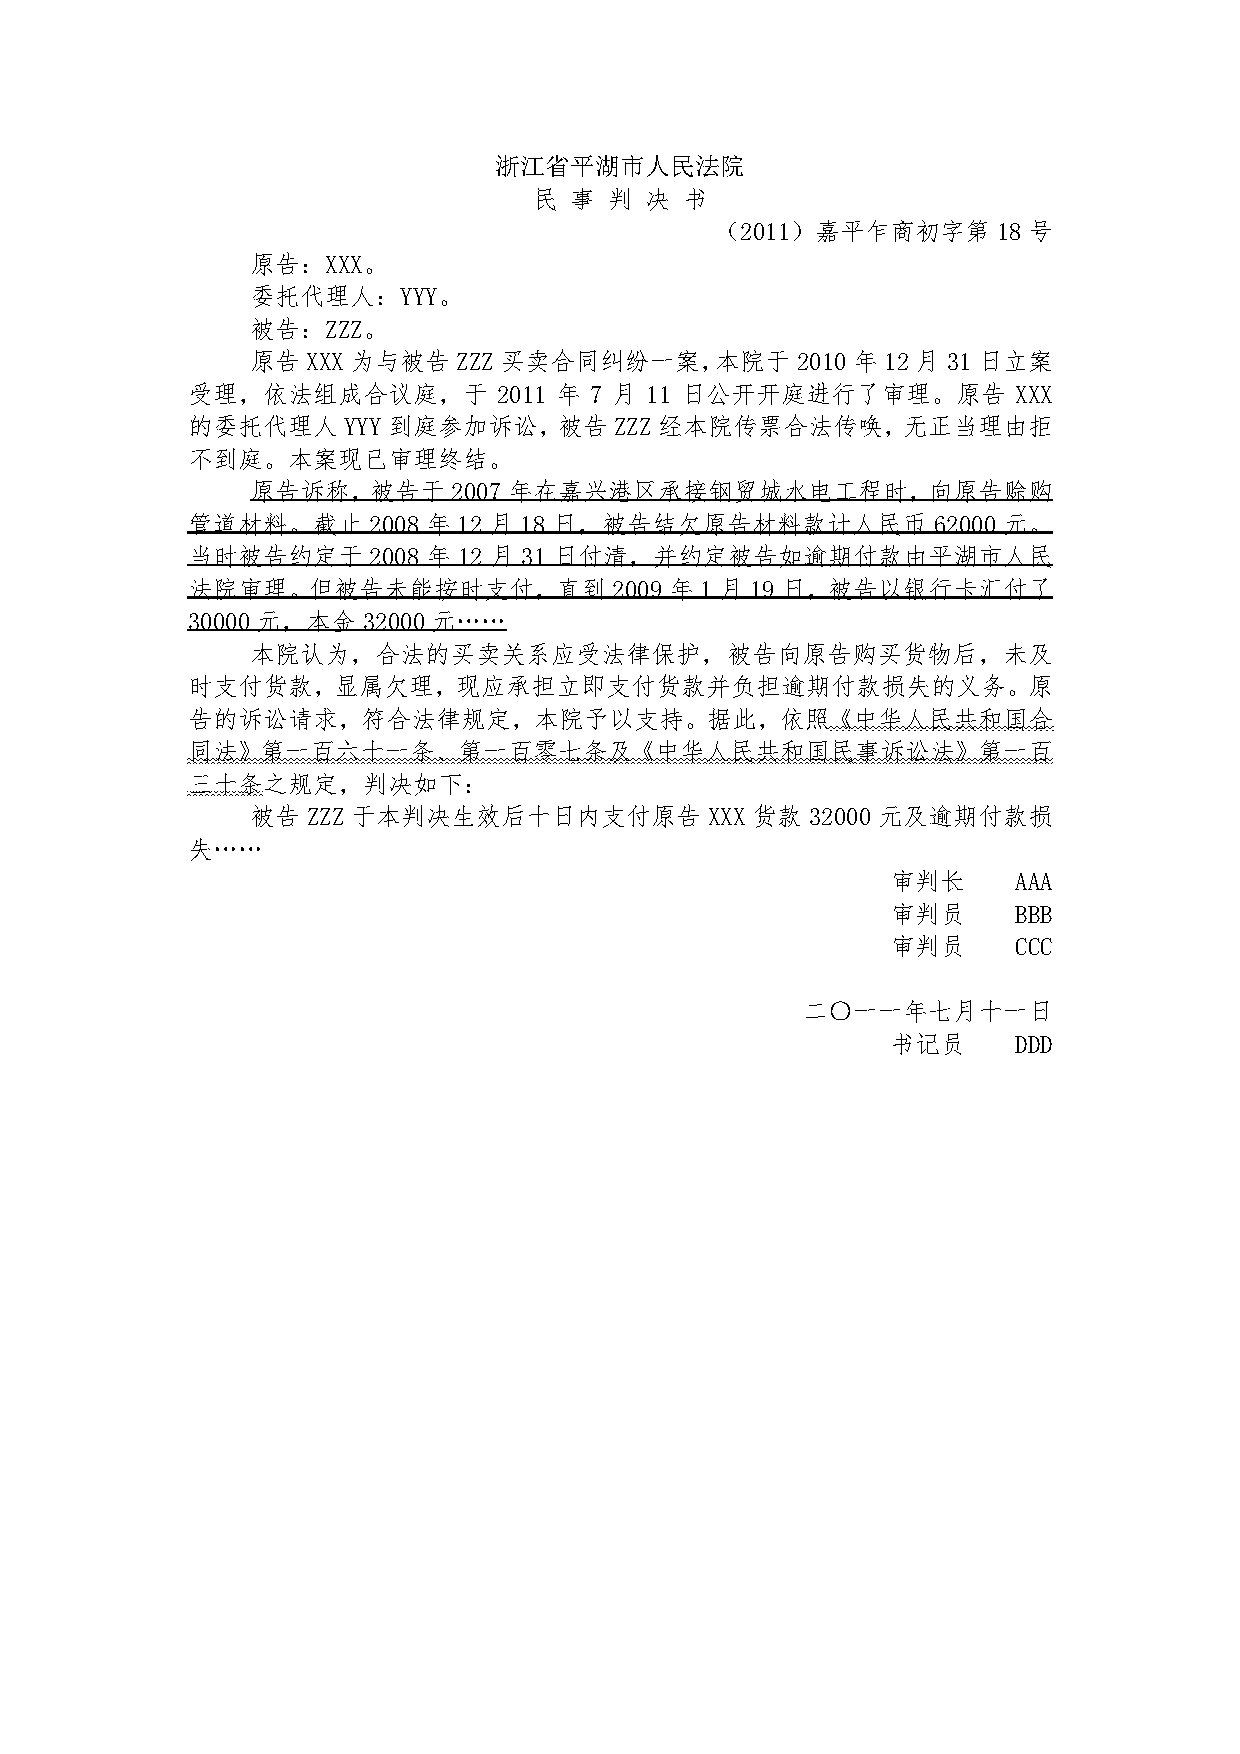
\includegraphics[width=10cm]{Figure2}\\
        \caption{测试用例拓扑图}\label{Figure2}
    \end{figure}

    在Engine 开始运行之前,需要为每个进程分配开始事件,并加入到Engine 的事件列表里。启动Engine,系统便会开始处理这些开始事件,使得所有进程开始工作,之后进程间就会开始进行信息的交互,直至生成树构建完毕。算法的执行结果如图\ref{SpanningTreeResult}左侧所示,相应的,我们构建了如图\ref{SpanningTreeResult}右侧所示的DFS 生成树。
    \begin{figure}[ht]
        \centering
        % Requires \usepackage{graphicx}
        \includegraphics[width=12cm]{SpanningTreeResult}\\
        \caption{测试用例结果图}\label{SpanningTreeResult}
    \end{figure}

    \subsection{算法的运行流程}
    为了更为清晰地展示DAPro 平台的工作原理,下面我们开始分析上述算法在DAPro 系统上的运行流程,如图\ref{Sequence}所示。

    \begin{figure}[ht]
        \centering
        % Requires \usepackage{graphicx}
        \includegraphics[width=14cm]{figures/Sequence}\\
        \caption{DAPro 顺序图}\label{Sequence}
    \end{figure}

    经过一系列的初始化动作,系统拓扑的构建、SpanningTreeProcess 对象的初始化都已完成,这时启动Engine,即调用Engine 的run 方法。根据run 方法的执行逻辑,Engine 会从事件列表中取出优先级最高的事件,即初始事件startP1,调用其action 方法执行。进程对象p1 是startP1 事件的执行实体。假设执行过程中p1 试图向另一个进程p2 发送消息,那么它将组装消息,并调用MessagePassingCom 类中的send2 方法将其发送给p2。MessagePassingCom 类中的dispatch 方法会找到相应的session,消息逐层被交付到相应的Link、Connector 对象,在完成传输过程后最终被交付到p2。p2 接收到消息事件后,就可以对其进行适当的处理。

%% !Mode:: "Tex:UTF-8"
\chapter{一个具体的协商算法及其在DAPro 平台的实现}
    本章我们将要利用DAPro 平台实现一个具体的协商算法\cite{fischer1983consensus}。我们将首先介绍协商问题的基本概念,然后描述和分析一个具体的协商算法,进而阐述如何在DAPro 中实现它,并测试实现的正确性。

    \section{协商问题}
    考虑一个系统,其中每个处理器$p_i$ 都有特殊的状态部件$x_i$,即输入,和$y_i$,即输出,也叫做决定。初始时,$x_i$ 保存了可能的输入中一些良序集合中的一个值,而$y_i$ 没有定义。任何对于$y_i$ 的赋值都是不可逆转的。对于协商问题的一个解决方案必须保证如下规则:
    \begin{description}
      \item[$Termination:$] 在每个可容许执行中,对于每一个没有发生故障的处理器$p_i$,$y_i$ 最终都会被赋予一个值。
      \item[$Agreement:$] 在每个执行中,对于所有没有发生故障的处理器$p_i$ 和$p_j$,如果$y_i$ 和$y_j$ 被赋值,那么必有$y_i=y_j$。也就是说,没有发生故障的处理器所达成的决定不会是冲突的值。
      \item[$Validity:$] 在每个执行中,如果对于一些值$v$,所有的处理器$p_i$ 都有$x_i=v$,那么对于一些没有发生故障的处理器$p_i$,如果$y_i$ 被赋值,有$y_i=v$。这就是说,如果所有处理器有相同的输入,那么在此基础上达成的决定必须为那个共同的输入。
    \end{description}

    注意一旦一个处理器崩溃了,那么算法将不再考虑该处理器,其决定也将没有任何限制\cite{attiya2004distributed}。

    \section{一个具体的协商算法}
    我们要实现的算法的伪代码描述如下所示。在算法中,每个处理器保存了它所知的一个值的集合,这些值都是系统中存在的。初始时,这个集合只包含了该处理器自己的输入。在接下来的周期中,一个处理器会通过合并从其他处理器接收的集合来更新其自身值的集合,同时会向其他所有处理器广播其集合中任何新加入的元素。这一过程将持续$f+1$ 个周期。 在第$f+1$ 个周期,处理器将选择集合中的最小元素作为决定。
    \begin{algorithm}[ht]
    \caption{Consensus algorithm in the presence of crash failures: \protect \\code for processor $p_i$, $0 \leq i \leq n-1$.}
    Initially $V$ = \{$x$\} \tcp*[f]{V contains $p_i$'s input}\\
    \BlankLine
    round k, $1 \leq k \leq f+1:$\\
    ~~~~send \{$v \in V: p_i$ has not already sent v\} to all processors\\
    ~~~~receive $S_j$ from $p_j$, $0 \leq j \leq n-1, j \neq i$\\
    ~~~~$V := V \cup \bigcup_{j=0}^{n-1}{S_j}$\\
    ~~~~if $k = f+1$ then $y$ := min($V$) \tcp*[f]{decide}\\
    \end{algorithm}

    \section{算法分析}
    我们可以清楚地看到,该算法恰好需要$f+1$ 个周期才能终止。更进一步地,Validity 条件很明显是满足的,因为决定的值都是某些处理器的输入。我们下面要证明算法满足Agreement 条件。

    根据Agreement 条件的定义,我们要证明对于任意两个没有发生故障的处理器$p_i$ 和$p_j$,在第$f+1$ 个周期结束时,都有$V_i=V_j$;这相当于证明在第$f+1$ 个周期结束时,若有$x \in V_i$,也就有$x \in V_j$。
    \begin{figure}[ht]
        \centering
        % Requires \usepackage{graphicx}
        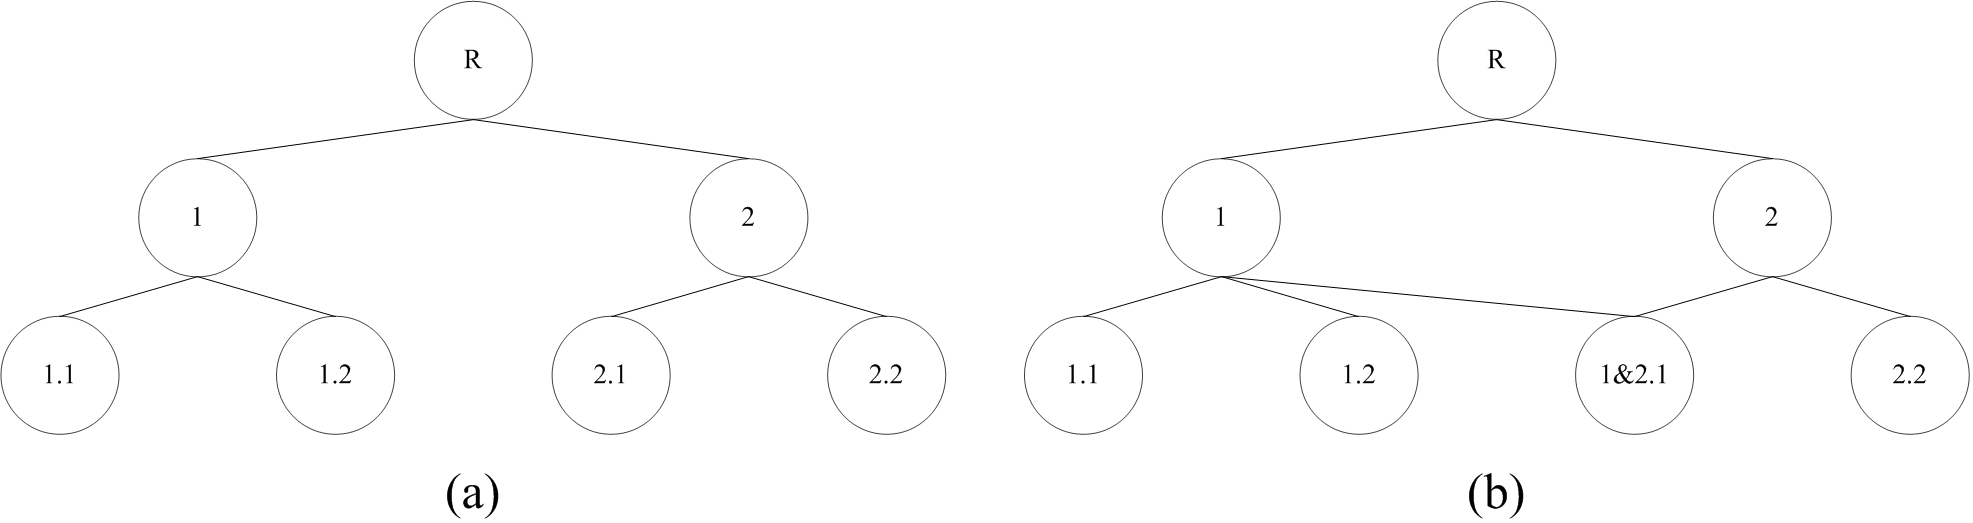
\includegraphics[width=10cm]{figures/Figure3}\\
        \caption{$f=3$ 时算法证明图示}\label{Figure3}
    \end{figure}

    对于任意正常状态下的处理器$p_i$,令$r$ 为$x$ 加入到$V_i$ 的第一个周期。如果$x$ 初始时就在$V_i$ 中,那么$r$ 值为$0$。 如果$r \leq f$,那么在第$r+1 \leq f+1$个周期,$p_i$ 会将$x$ 发送给每个$p_j$,这就使得$p_j$ 将$x$ 加入到$V_j$(如果$x$ 不是已经在$V_j$ 中)。

    否则,假定$r=f+1$,并且令$p_j$ 为在第$f+1$ 个周期首次接收到$x$ 的一个正常状态下的处理器。那么必然有一个含有$f+1$ 个处理器的链$p_{i_1},...,p_{i_{f+1}}$ 将值$x$ 传递给$p_j$。 也就是,在第$1$ 个周期,$p_{i_1}$ 将$x$ 发送给$p_{i_2}$,在第$2$ 个周期,$p_{i_2}$ 将$x$ 发送给$p_{i_3}$,以此类推。最后在第$f$ 个周期,$p_{i_f}$ 将$x$ 发送给$p_{i_{f+1}}$;在第$f+1$ 个周期,$p_{i_{f+1}}$ 将$x$ 发送给$p_j$。(图\ref{Figure3} 给出了$f=3$ 的情况。)由于对于一个特定的值每个处理器只发送一次,处理器$p_{i_1},...,p_{i_{f+1}}$ 形成了一个含有$f+1$ 个不同处理器的集合。因此,在$p_{i_1},...,p_{i_{f+1}}$ 中至少有一个正常状态下的处理器。但是,这个处理器在某个$\leq f < r$ 的周期将$x$ 加入其集合中,这与$r$ 是最小的假定相矛盾。

    因此,所有没有发生故障的处理器在第$f+1$ 个周期都有相同的本地集合,因而其决定的值是相同的。这就证明了Agreement 条件是满足的\cite{attiya2004distributed}。

    综上,我们证明上述算法能够在存在崩溃故障的情况下,在$f+1$ 个周期内解决协商问题。

    \section{算法实现}
    为实现上述协商算法,我们在DAPro 系统中定义了ConsensusProcess 类为该算法的参与实体。ConsensusProcess 类继承了Process 类,覆盖了其run 方法,并增加了算法所需的很多额外信息,其类图如图\ref{ConsensusProcess} 所示。
    \begin{figure}[ht]
        \centering
        % Requires \usepackage{graphicx}
        \includegraphics[width=14cm]{figures/ConsensusProcess}\\
        \caption{ConsensusProcess 类图}\label{ConsensusProcess}
    \end{figure}

    ConsensusProcess 类中定义了数据成员localSet 表示保存在本地的值的集合,unsentSet 表示尚未发送的值的集合,两者均为HashSet 类型。由于算法的实现需要对多种事件进行处理,我们定义了receivedEvent 表示ConsensusProcess 对象需要处理的事件,这些事件包括消息传递RoundEvent 事件、本地计算RoundEvent 事件和消息事件。在一个周期中,当ConsensusProcess 对象处理消息事件时,需要将接收的消息保存在消息链表receivedMessage 中,这是该进程对象在该周期接收到的消息的集合。最后,ConsensusProcess 对象达成的决定保存在数据成员decision 中。

    算法的主要逻辑由ConsensusProcess 类中的run 方法实现。对于不同类型的事件,run 方法的处理方式如下:
    \begin{description}
      \item[MessagePassingRoundEvent] 如果进程对象接收到的是MessagePassingRoundEvent,那么这代表着一个周期的开始。此时我们利用FailureGenerator 模块随机产生故障,即改变进程对象的状态为故障状态。之后我们会对进程对象的状态进行判断:如果为正常状态,那么进程对象会将unsentSet 中的内容组装成消息发送给其他所有进程;如果该进程对象刚刚发生故障,那么进程对象会随机地将unsentSet 中内容的全部或者一部分发送给其他进程,每个进程接收到的值的集合可能各不相同;如果该进程对象已经在上一个周期发生故障,那么将不会有消息发送。
      \item[LocalComputationRoundEvent] 如果进程对象接收到的是LocalComputationRoundEvent,那么如果该进程对象是正常状态,那么就会进行一次本地计算,即根据接收到的消息对localSet 进行更新并筛选出其中未被发送的值加入到unsentSet中,进程对象在一个周期中接收的消息都保存在receivedMessage 中,receivedMessage 中的内容会在一个周期结束后清空。在第$f+1$ 个周期,所有的进程对象都会遍历localSet 集合,选择其中最小的值作为其决定的值。
      \item[MessageEvent] 如果进程对象接收到的是消息事件,那么我们需要从消息事件中取出消息,加入到进程对象的receivedMessage 中。消息的处理过程需要等进程对象接收到相应的RoundEvent 事件时触发。
    \end{description}

    针对该算法,我们重新定义了一种消息类型ConsensusMessage,它是Message 类的子类,其类图如图\ref{ConsensusMessage}。ConsensusMessage 类中包含数据成员content 及其get 和set 方法,其中content 是一个集合,与ConsensusProcess 中的数据成员localSet 和unsentSet 的类型相一致。
    \begin{figure}[ht]
        \centering
        % Requires \usepackage{graphicx}
        \includegraphics[width=12cm]{figures/ConsensusMessage}\\
        \caption{ConsensusMessage 类图}\label{ConsensusMessage}
    \end{figure}

    此外我们定义了ConsensusAction 类对算法中的不同类型事件进行处理。ConsensusAction 实现了IProcessAction 接口并实现了其中的execute 方法:调用ConsensusProcess 类的setEvent 方法将事件保存在其数据成员receivedEvent 中,之后调用其run 方法启动进程。

    \section{运行结果分析}
    通过建立包含五个ConsensusProcess 对象的测试用例,我们对算法实现的正确性进行验证。根据Consensus 问题的假定,系统拓扑是一个完全图,也就是任意两个进程对象之间都有双向信道。我们按照图\ref{Figure4}创建系统拓扑。
    \begin{figure}[ht]
        \centering
        % Requires \usepackage{graphicx}
        \includegraphics[width=10cm]{figures/Figure4}\\
        \caption{测试拓扑图}\label{Figure4}
    \end{figure}

    完成了系统初始化工作后,我们根据系统可允许发生故障处理器个数的不同,测试算法解决协商问题需要的周期数。测试结果会给出各个进程对象的状态以及本地集合localSet 和决定的情况。

    当系统可允许发生故障处理器的个数为$1$(即系统是$1-resilient$ 的)时,一个周期后算法执行结果如图\ref{ConsensusResult1} 所示。

    \begin{figure}[ht]
        \centering
        % Requires \usepackage{graphicx}
        \includegraphics[width=6cm]{figures/ConsensusResult1}\\
        \caption{$1-resilient$ 系统中算法执行一个周期的结果}\label{ConsensusResult1}
    \end{figure}

    从结果中可以看到,编号为2、3、4、5的进程都处于正常状态(正常状态用0 表示),但是其本地集合localSet 和决定值decision 并不都相同。通过输出更多的程序执行信息我们发现,编号为1 的进程发生故障(用2 表示),从而导致发送给2、3、4、5 号进程的消息不都相同,2、4、5号进程接收到了值“1”而3号进程并没有。因为一个周期之后四个正常状态的进程的决定值不同,所以四者没有达成一致的决定,也就是协商问题未能在一个周期内解决。接下来,我们增加一个周期进行测试,其结果如图\ref{ConsensusResult2}所示。
    \begin{figure}[ht]
        \centering
        % Requires \usepackage{graphicx}
        \includegraphics[width=6cm]{figures/ConsensusResult2}\\
        \caption{$1-resilient$ 系统中算法执行两个周期的结果}\label{ConsensusResult2}
    \end{figure}

    在增加了一个周期后,算法执行的结果发生了改变。发生故障的进程依然是一个,但是处于正常状态的所有进程的本地集合是相同的,因而四者达成了一致的决定。而对于发生故障的进程,我们对其决定的值不作考虑。注意尽管系统中最小的输入是1,但是由于进程1 发生故障并且没有将值“1” 发送给其他任何进程,因而最终其他进程达成的决定值为2 是合理的。

    我们适当提高系统的容错能力,将系统可允许发生故障处理器的个数置为$2$(即系统是$2-resilient$ 的),分析两个和三个周期后算法执行的结果。算法执行两个周期的结果如图\ref{ConsensusResult3}所示。
    \begin{figure}[ht]
        \centering
        % Requires \usepackage{graphicx}
        \includegraphics[width=6cm]{figures/ConsensusResult3}\\
        \caption{$2-resilient$ 系统中算法执行两个周期的结果}\label{ConsensusResult3}
    \end{figure}

    很明显,2、3、4 号进程处于正常状态,而1、5 号进程发生了故障。然而2、3、4 号进程的localSet 和decision 并不相同,也就是在两个周期内算法未能解决协商问题。分析算法执行过程可以发现1 号进程在第一个周期发生故障,并且只将值“1”发送给5 号进程;而在第二个周期,5 号进程恰好发生故障,将值“1”发送给了2、4 号进程,因此3 号进程没有接收到值“1”,从而导致了决定值的不一致。同样的,我们增加一个周期进行测试,算法执行结果如图\ref{ConsensusResult4}所示。
    \begin{figure}[ht]
        \centering
        % Requires \usepackage{graphicx}
        \includegraphics[width=6cm]{figures/ConsensusResult4}\\
        \caption{$2-resilient$ 系统中算法执行三个周期的结果}\label{ConsensusResult4}
    \end{figure}

    三个周期后,处于正常状态的三个进程的localSet 和decision 都达成了一致。也就是对于$2-resilient$ 系统,算法需要三个周期才能解决协商问题,这与我们算法分析部分的结果相一致。

    根据对上述测试结果的分析,我们证实了上文对于算法的分析,也就是算法能够在系统存在$f$ 个故障的情况下在$f+1$ 个周期内解决协商问题,同时也验证了算法实现的正确性。

%% !Mode:: "Tex:UTF-8"
\chapter{总结与未来工作}
    分布式算法出现在很多领域的应用中,包括电信、分布式信息处理、科学计算和实时进程控制。为这些应用构建分布式系统的重要一步工作就是分布式算法的设计实现和分析。本文主要研究一个针对分布式算法的原型模拟平台$\pozhehao$DAPro。论文前面部分已经详细讨论了我们的工作,下面我们对本文工作做一个总结,并展望未来工作的方向。

    \section{工作总结}
    本文首先简述了分布式算法及其原型实现的概念,介绍了论文的背景。然后概括了其他网络模拟平台和离散事件模拟方面的相关工作,分析了其与本文工作的区别和联系。之后,我们阐述了论文的基础理论知识,对分布式计算模型进行了系统分析。论文的主要部分是DAPro 平台的设计与实现,以及基于DAPro 平台两个分布式算法的实现与分析。总的来看,本文的主要工作包括以下几个方面:
    \begin{itemize}
      \item 详细阐述了DAPro 平台的设计实现。总体概述描述了DAPro 平台的模块结构和运行流程,模块设计部分对平台每个模块的功能和实现进行了详细分析,并以一个DFS 生成树的构建算法为例描述了如何使用DAPro 平台实现一个分布式算法,展示了平台运行算法的流程。
      \item 在原始框架的基础上对DAPro 平台的功能进行了大量扩充。本文在DAPro 平台原始框架的基础上增加了更为丰富的Connector 类型、更多的事件和进程类型、更多的事件动作,并增加了故障生成等模块,提高了系统对于分布式算法的模拟能力。
      \item 基于DAPro 平台实现了分布式的DFS 生成树构建算法和可容错的协商算法。通过具体的实验和对结果的分析,验证了DAPro 平台的正确性和可用性。
    \end{itemize}

    \section{未来工作}
    目前我们已经设计实现了DAPro 平台的系统框架,并在此基础上实现了一些基本的算法,验证了平台的可用性。未来我们的主要工作是要继续优化DAPro,使其成为一个完整而实用的分布式算法模拟平台。具体来说,我们的未来工作包括以下方面:
    \begin{itemize}
      \item 优化DAPro 平台的结构设计。目前DAPro 平台的模块划分(主要是System 模块)尚存在一些疑问,一些模块的实现也并不完整,还有一些功能可以简化。接下来我们将进一步优化DAPro 系统的结构,实现更为清晰的模块划分。
      \item 完善FailureGenerator 模块的设计。目前DAPro 产生故障的逻辑还很原始,是采用直接修改进程状态的方法。为了符合离散事件模拟的思想,我们将增加故障事件,模拟系统中可能出现的各类故障,不仅包括目前所实现的简单崩溃故障,还有拜占庭故障;不仅包括进程发生故障的情况,还应该有信道发生故障的情况。
      \item 更多功能的实现。目前我们已经可以利用DAPro 平台来模拟一些简单的分布式算法,但是这还远远不够。进程间的通信不光可以采用消息传递模型,也可以通过共享变量的方式;平台可以对算法运行数据进行统计;使用XML 文件配置系统拓扑;为平台设计GUI 等都是我们接下来试图达到的目标。
      \item 编辑用户手册。目前DAPro 平台尚无系统的用户手册供读者参考,接下来我们除了继续推进DAPro 的设计实现,还将编辑整理用户手册,提高系统的可读性。
    \end{itemize}

\backmatter
\pagenumbering{Roman}

% 参考文献
\bibliographystyle{unsrt}
\bibliography{ref/reference}
\addcontentsline{toc}{chapter}{参考文献}
% 致谢
% !Mode:: "Tex:UTF-8"
\chapter*{致\qquad 谢}
\addcontentsline{toc}{chapter}{致谢}

毕业论文写到这儿,算是接近尾声了。同样接近尾声的,还有我本科的四年时光和我的青春。在这论文最不醒目的位置,我想郑重地感谢在毕业论文撰写过程中帮助过我的老师和同学,同时还要感谢在过去四年支持我、陪伴我的亲人朋友们。

首先要感谢的是我的指导老师黄宇副教授。过去近一年时间,在他的悉心指导下,我除了完成毕业论文,也对科研态度和方法有了初步的认识。黄老师在学术上严谨,在生活中随和,很荣幸接下来三年研究生期间能继续有他的指导和教诲。

此外还要感谢魏恒峰师兄、杨怡玲师兄、陆掾师兄以及江雪、王少萍、王琨同学在论文撰写过程中给予我的帮助和支持。感谢这四年陪伴我的舍友,曾经一起欢笑的同学朋友,还有那些我倾心的女孩,是他们让我度过了意义非凡的四年,感谢这一路的陪伴。

最后要衷心感谢我的父母,是他们辛勤的付出让我没有生活的负担,可以安心投入学习和工作中去。我将尽我全力报答他们的养育之恩!



\end{document}
